\documentclass{amsart}
%\documentclass[epsf]{article}
\usepackage{framed}
\usepackage{graphicx}



\usepackage{parskip,newclude}
\usepackage[margin=1in]{geometry}
\setlength{\parindent}{15pt}



\usepackage{setspace,fancyhdr}
\pagestyle{fancy}
\fancyhead[L]{{\scshape }}
\fancyhead[R]{{\scshape }}


\begin{document}
\title{Optimizing the Boston Emergency Medical Services Shift Schedule}

\author{(Tam Nguyen, Wesley Cai) \\
Faculty advisor:  Rachel Maitra (WIT) \\
Applied Mathematics, Wentworth Institute of Technology, Boston, MA, USA}

\maketitle

\onehalfspacing 

%\include*{ProjectSummary}
%\include*{Reference}


\section{Abstract} 
We present a method to optimize a shift schedule for each station as well as finding the most optimal way to place paramedics and ambulances at stations located in and around the Boston metropolitan area. The goal is to minimize the need for ambulances during a specific time period, given a certain expected coverage. Using data received from the Boston Emergency Services regarding the number of incidents per hour in a day, we generated a demand curve for our study area Roxbury. We plan to use the model of the study area to analyze other parts of Boston. The end goal is to compare our model with the linear model in Ragopalan et. al paper Ambulance Deployment and Shift Scheduling: An Integrated Approach. Our final results were produced from a simulation that was ran 10,000 times which represent the simulated days. It gave us a random the number of calls per day and a random number of ambulances that would be needed. We ran the code in R, which is a statistical program.

\noindent Keywords: \\
Shift Scheduling, Optimization, Boston Emergency Medical Services, Roxbury

\section{Introduction}

Emergency medical services (EMS) can be expensive in large cities such as Boston and Los Angeles [4]. Historically, EMS regulations were only established in the early 1970s. Before then, the only pre-hospital care people received were transportation. To cut costs, funeral homes played an important part in providing service and transportation [4]. Labor costs tend to be the single greatest component of providing EMS [4]. In 2013, the Boston EMS provided 142, 341 support units including basic life support (BLS) and advanced life support (ALS). Surprisingly enough, there were only 24 frontline ambulances (19 EMT and 5 paramedic) available serving a population of about 645,000 [2]. This indicates that a change in shift schedule has a great impact on the efficiency of the Boston EMS (City of Boston). Therefore, we would like to investigate how a change in the shift schedule will affect the performance of the current Boston EMS system. More specifically, this thesis deals with optimizing a shift schedule to find the best way to place paramedics and ambulances at stations located in and around the Boston metropolitan area. By stations, we mean where the ambulances are located at a specific time of day. The 2013 Boston EMS data will help us determine which station to focus on initially. In order to provide the best care, the EMTs and paramedics must respond to calls in an efficient manner and timely manner. \\

The first stage will consist of picking a study area to concentrate on. A shift schedule must satisfy some constraints such as the max number of shifts people can work or the max number of hours worked per day. After the shift schedule is determined, the model should optimize the number of ambulances that are in service per hour. In detail the decision variables of a shift schedule model will include the length of each shift ( 8 or 10 hours shifts), start time of each shift, and the number of different shifts that will be needed based on minimizing the number of ambulances. The second stage consists of creating a simulation that will randomly generate the number of calls a region receives per hour as well as randomly selected times that a call would be received.\\

This paper is organized as follows. Section 3 contains the information on what has previously been done relating to shift schedules of paramedics and ambulances. Section 4 presents the Information and Data which discussed how the data and information was gathered as well as the plots. Section 5 discussed the model and results of optimizing the shift schedule. \\


\section{History}

Church et al. [5] created a model that closely resembles our goal [5]. Their models goal was to schedule shifts in a way that closely matched the fluctuating incidents over each day of the week. They included visuals such as graphs that depicted the number of units scheduled in a given hour. The authors realized that in order for their model to be successful they must deploy EMTs and paramedics as close as possible to the unit demand curve, which is the curve that describes the number of ambulance units needed per hour [5]. This model used discrete integer programming.

Rajagoplan et al. [3] attacked this problem in two steps. First, he created a dynamic expected coverage model, and figured out the minimum number of ambulances for each time interval, given certain coverage requirement of each time interval and locations. Second, with the solution from the first step, Rajagoplan et. al [3] developed a different model to determine the optimal shifts. Since the first model can not be solved by
integer linear programing, the authors stated that a heuristic algorithm and a tabu search, might be possibly utilized to solve the model due to the structure of the problem [3]. One of the most admiring parts of this paper is that the results, which consist of tables and maps can be easily understood. \\

\section{Information and Data}

Recently, we spoke to someone from the Boston Emergency Services and he provided us with information about the average number of incidents by hours per day. He also provided us with information on how they currently schedule shifts for their staff. Once the frequency chart (provided with average number of incidents by hours) was received, we generated a demand curve for our study area, Roxbury. Roxbury was chosen as the study area because it was one of the regions in Boston with the most incidents in 2013 [1].

Our first task was to gather data on the Boston Emergency Medical Services regarding the call volume/number of incidents per hour. Figure 1. from above represents the call volume for the City of Boston. Using this demand curve, we used it to find the call volume per hour for Roxbury (Figure 2) based on Figure 1. Since Roxbury had a high number of incidents in 2013 and we thought it would be a good way to test our model. Our study area will then expand to other regions in Boston. We?re going to compare our model to the Paper Model, which assigns one ambulance to each incident/call. For multiple regions in Boston, we are assuming that ambulances closer to other regions can go take care of incidents in those regions. Ambulances are also prioritized based on the region that they are in, for example if there all the ambulances in Roxbury are occupied, then Roxbury will have to borrow an ambulance from a surrounding region that does not have a high call volume. The point is to not borrow an ambulance from a region that has a higher call volume during that time. 

%$$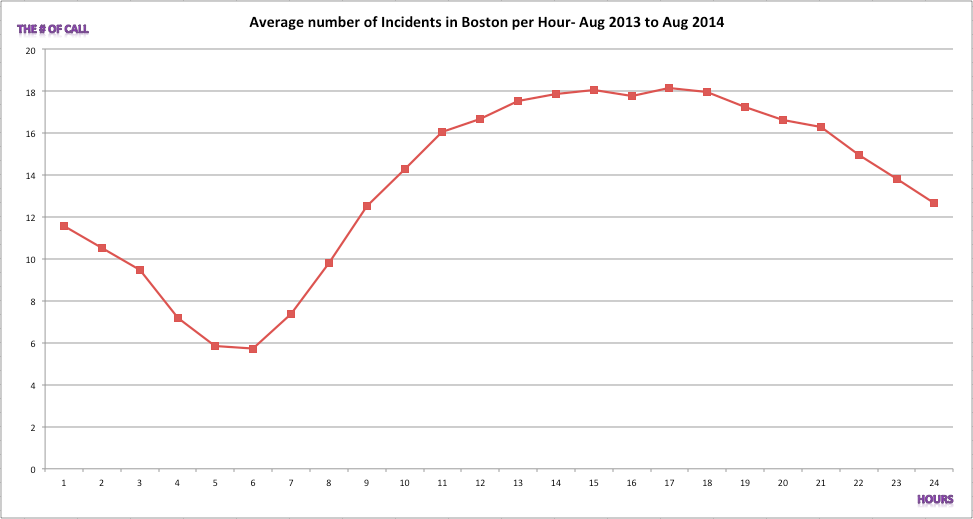
\includegraphics[scale=0.45]{theDemandCurveForBoston.png}$$
%\indent Figure 1. This is the demand curve for the call incidents per hour per day.\\
%$$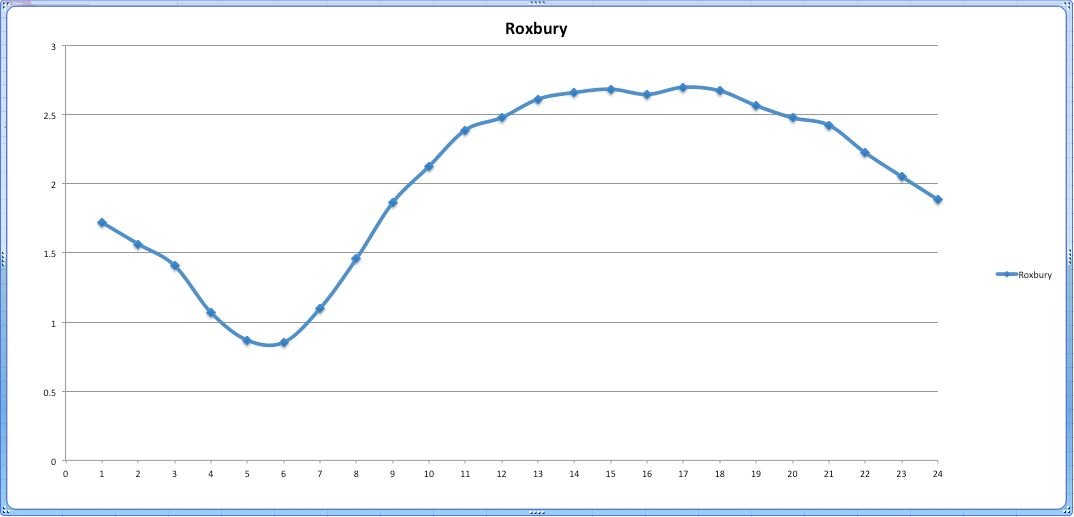
\includegraphics[scale=0.4]{Roxbury_Demand_Curve.png}$$
%\indent Figure 2. This is the demand curve for the call incidents per hour per day.\\

%$$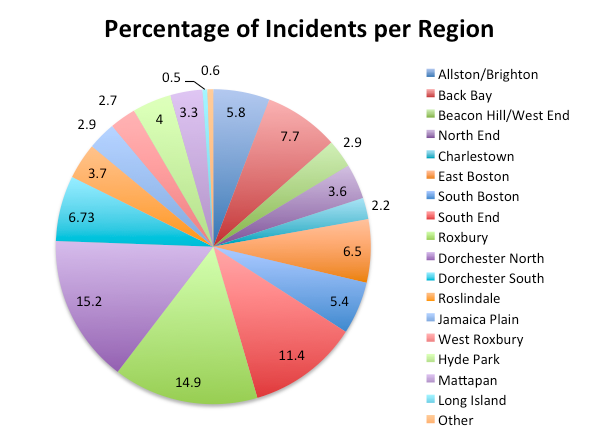
\includegraphics[scale=0.6]{Percentage_of_incidents.png}$$
%Figure 3. This graph represents the percentage of incidents per region in Boston. From this you can see that the areas with the most number of incidents were Roxbury, Dorchester North, and South End. \\

%$$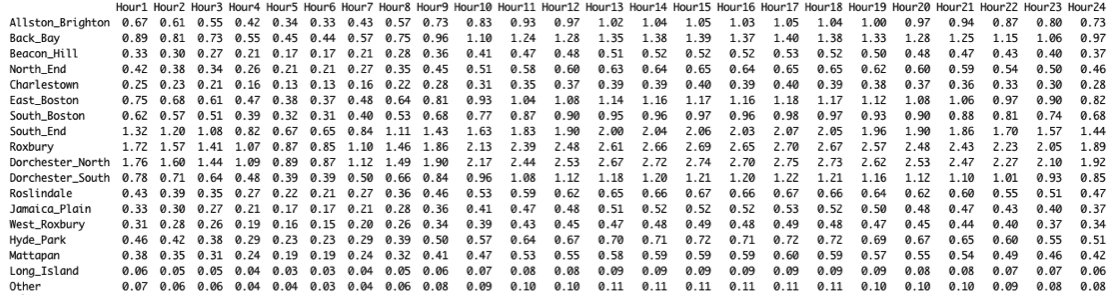
\includegraphics[scale=0.9]{hourperregion.png}$$
%Figure 4. This was derived from the demand curve of Boston and the Percentage of Incidents chart.
%$$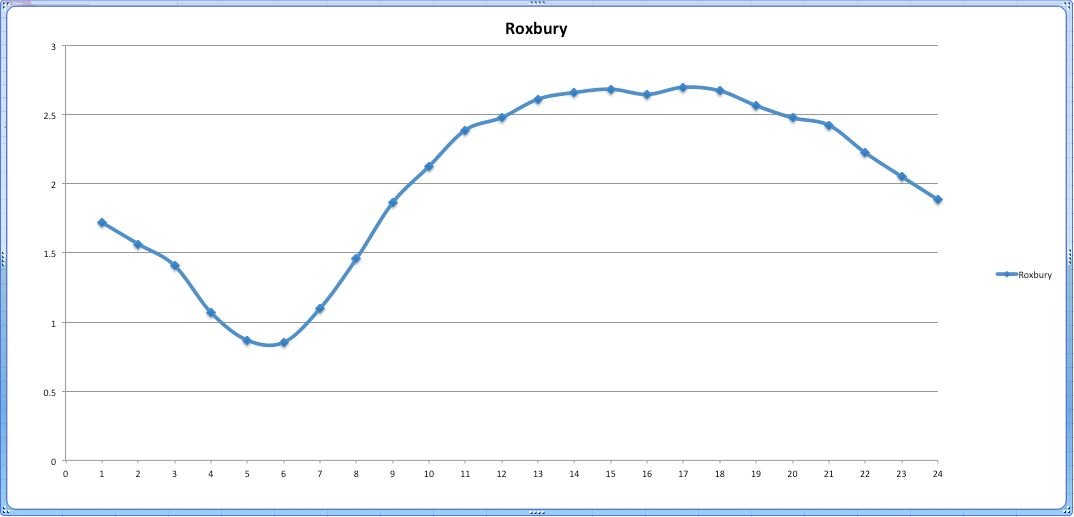
\includegraphics[scale=0.4]{Roxbury_Demand_Curve.png}$$

\section{Model \& Results}

Our model is compared to the Paper Model which assigns one call to one ambulance. This is not efficient because if you have ten calls then you would need ten ambulances to take care of each incident. 

The assumptions for the model are:
\begin{enumerate}
\item The number of calls / incidents follows Poisson distribution.
\item The moments of calls is uniformly distributed. Ex.  P(a call at 11:05) = P(a call at 11:38) .
\item The service time for an ambulance is fixed by 20 minutes. In other words, how long it takes an ambulance becomes available after heading out from ambulance station is 20 minutes.      
\end{enumerate}

%$$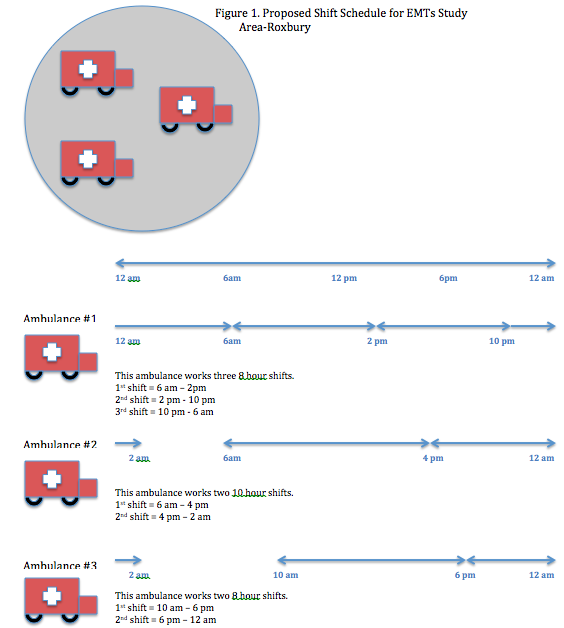
\includegraphics[scale=0.5]{Figure1.png}$$
%Figure 4. This is a shift schedule for Roxbury using three ambulances since that is the maximum number of ambulances needed in a 24 hour period. Refer to the Figure 2 to see the demand curve.


Since the study area is Roxbury, we will focus on one hour time period (11 a.m. to 12 p.m.) to test our model. The model will Generate a random number that follows Poisson distribution with mean 2.39. It stands for the number of incidents occurring during 11 am to 12 pm in Roxbury. Suppose the first random number is 5. It stands for five 911 calls, which require five ambulances between 11 am and 12 pm. Given there are 5 calls, we generate 5 moments for the calls occurring ``5,12,20,38,50'' which stand for 11:05, 11:12, 11:20, 11:38, and 11:50. Since the service time for an ambulance is 20 minutes, an ambulance can take care of three calls at most within an hour. Calls at 11:05, 11:12, 11:20, 11:38, and 11:50, we have:
%$$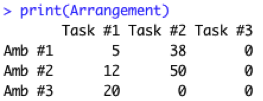
\includegraphics[scale=1]{PrintArrange.png}$$
The first call at 11:05 was assigned to the ambulance \#1, and the second call at 11:12 could not be assigned to the ambulance \#1, because the ambulance \#1 is still taking care of the first call. So the ambulance \#2 has to take the second call at 11:12. Similarly, 11:20 has to be assigned to the ambulance \#3, because the ambulance \#1 and \#2 were not available.  At 11:25, the ambulance \#1 became available, so it can take the task of the third call at 11:38. For the last call at 11:50, the ambulance \#2 can take it. Therefore, in order to let a patient being assigned an ambulance immediately without waiting, we need to allocate three ambulances between 11 am and 12 pm in Roxbury.


Another experiment demonstrates (10 calls): Calls at 11:05, 11:12, 11:18, 11:20,11:25, 11:38, 11:42, 11:50,11:51, and 11:52.
%$$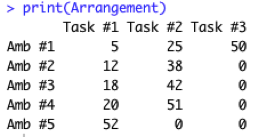
\includegraphics[scale=1]{PrintArrange2.png}$$
Based on the random 10 calls, in order to let a patient being assigned an ambulance immediately without waiting, we need to allocate five ambulances between 11 am and 12 pm in Roxbury. 

We simulated 10,000 days/tests which gave us the number of calls and number of ambulances needed, what is the performance with constant various number of ambulance supply.
Since the 10,000 rows is too long in this paper to show, we only presented first 10 tests and last 10 test of it.
%$$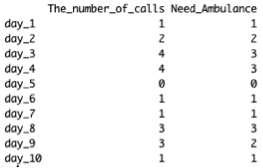
\includegraphics[scale=1]{numcalls.png}$$
%$$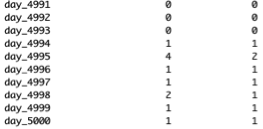
\includegraphics[scale=1]{numcalls2.png}$$


The number of calls column is following a Poisson distribution with a mean of 2.39. The Need Ambulance column indicates the number of ambulances needed is based on a no wait ratio. In fact, sometimes a patient cannot be assigned an ambulance immediately so they might have to wait a few minutes due to the limited number of ambulances and budget.

%$$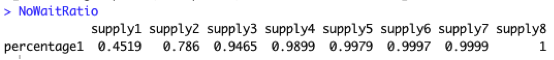
\includegraphics[scale=1.3]{Nowaitratio.png}$$

Supply1, Supply3, and Supply7 represents constantly supplying 1, 3, or 7 ambulances. Percentage1 is the probability that a patient is being assigned an ambulance immediately without waiting, given the constant supply of ambulances. From our 10,000 days/tests simulation, supplying 3 ambulances between 11 am and 12 pm in Roxbury has approximately 95\% that that a patient is being assigned an ambulance immediately, which is very high enough. Supplying 7 or 8 ambulances does not seem so reasonable, because the marginal cost is too high. Since there are 10,000 tests, the ?NoWaitRatio? or percentages are considered significant. Therefore, supplying 3 ambulances between 11 am and 12 pm in Roxbury is an ideal choice. 






From the demand curve showing the average calls per region, we can find the least supply number of ambulances that has 95\% confidence of a patient being assigned an ambulance immediately by using the same method as above.

%$$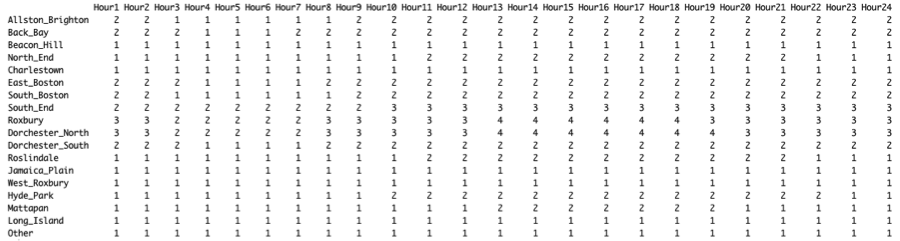
\includegraphics[scale=1.1]{supplytable.png}$$
Figure 5. This shows the number of ambulances needed per hour for all the regions in Boston within a 24 hour period.




%$$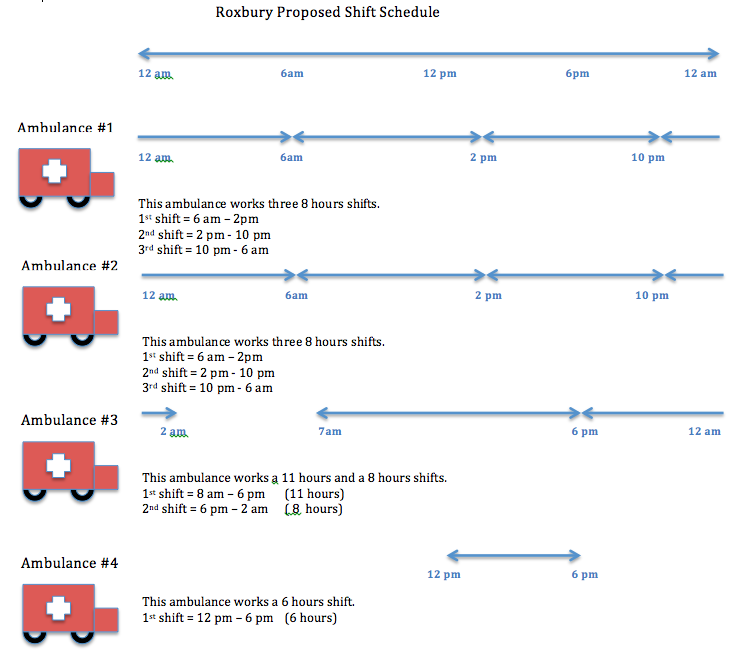
\includegraphics[scale=.55]{rox_sche.png}$$
Figure 6. In Figure 5, it shows that the maximum number of ambulances needed in a 24 hour period was four. So, Roxbury is assigned four ambulances. Ambulance 1 and Ambulance 2 both work for 24 hours with three 8 hours shifts, Ambulance 3 works for 19 hours with an 11 hour shift and an 8 hour shift, and Ambulance 4 works for 6 hours from 12 p.m. to 6 p.m.


\section{Acknowledgement}

We would like to thank Brendan Kearney who is the Superintendent in Chief of the Boston Emergency Medical Services. We had a phone interview with him early in the semester to ask him about the current shift schedule they have in place for paramedics and ambulances. He also gave us data which included the call volume per hour in a 24 hour time period. From this we generated a demand curve in Excel to give us more of visual interpretat

\section{Conclusion}

In this paper we have developed a solution approach to optimizing the shift schedule for the Boston Emergency Medical Services (EMS). Our result is based on the simulation of 10,000 times for each hour and region. The model minimizes the number of ambulances needed per region based on the fixed time of 20 minutes to respond to an incident before being assigned a new task. Our model also saves money because ambulances can have more than one task per hour, which makes it more efficient than the Paper Model where one task is assigned to a different ambulance. We may use Queuing theory as our approach to calculate the no-wait ratio and other values that represent the features of ambulance (Queuing) system, such as the expected waiting time (minutes) on average, or the distribution of waiting time after calling 911. In our model, the service time is fixed, which is not realistic. Therefore, the next step of this project is using a distribution to represent the service time that is not a fixed value. With this consideration, we believe than our model becomes more realistic and applicable.

The broader impact of this project is that it can be applied to various other emergency services such as fire departments, police departments as well as food delivery services, and UBER services. In the case if the fire and police departments, our model can be applied to them because it�s almost similar. Instead of having ambulances, you can change it to fire engines and police cruisers, and police officers and firefighters instead of EMTs and paramedics. And UBER is like a taxi service and the model can be applied in this instance because people call them for rides and generally wait for the drivers to pick them up. The model can still be applied because the UBER drivers would have to reach the person in a set amount of time.

%\section{Appendix}
%R Code

\newpage
\begin{thebibliography}{9}




\bibitem{City of Boston} City of Boston, Boston Emergency Medical Services, 2013 Vital Statistics.

\bibitem{City of Boston} City of Boston, Boston EMS Ambulances.


\bibitem{Shiah} D. Shiah, S. Chen. Ambulance allocation capacity model, (2007) 40-46.

\bibitem{Rajagopalan} H. Rajagopalan, C. Saydam, E. Sharer, and H. Setzler. Ambulance Deployment and Shift Scheduling: An Integrated Approach, Journal of Service Science and Management, (2011) 4, 66-78.

\bibitem{Church} R. Church, P. Sorensen, and W. Corrigan, Manpower Deployment in Emergency Services, (2001) 1-16, 37, 219-234.

\end{thebibliography}

\end{document}